\appendix
\part*{Annexes}
\addcontentsline{toc}{part}{Annexes}
\pagestyle{myheadings}
\markboth{Annexes}{Annexes}

Les annexes contiennent certaines illustrations du mémoire ainsi que la description des fichiers disponibles dans les livrables sur Github à cette adresse : \url{https://github.com/LaureRossignol96/MemoireTNAH2020}. 

Nous présentons d'abord les annexes qui illustrent le mémoire et auxquelles nous renvoyons explicitement dans le mémoire : ce sont les annexes A, B et C.

Les annexes D décrivent les livrables du CRHXIX, les annexes E ceux du Labex OBVIL.

\chapter{Édition numérique de correspondance}
\section{Exemples d'éditions déjà existantes}

\begin{figure}[H]
    \centering
    \caption{\emph{D'Alembert en toutes lettres}. Édition numérique de la correspondance de D'Alembert}
    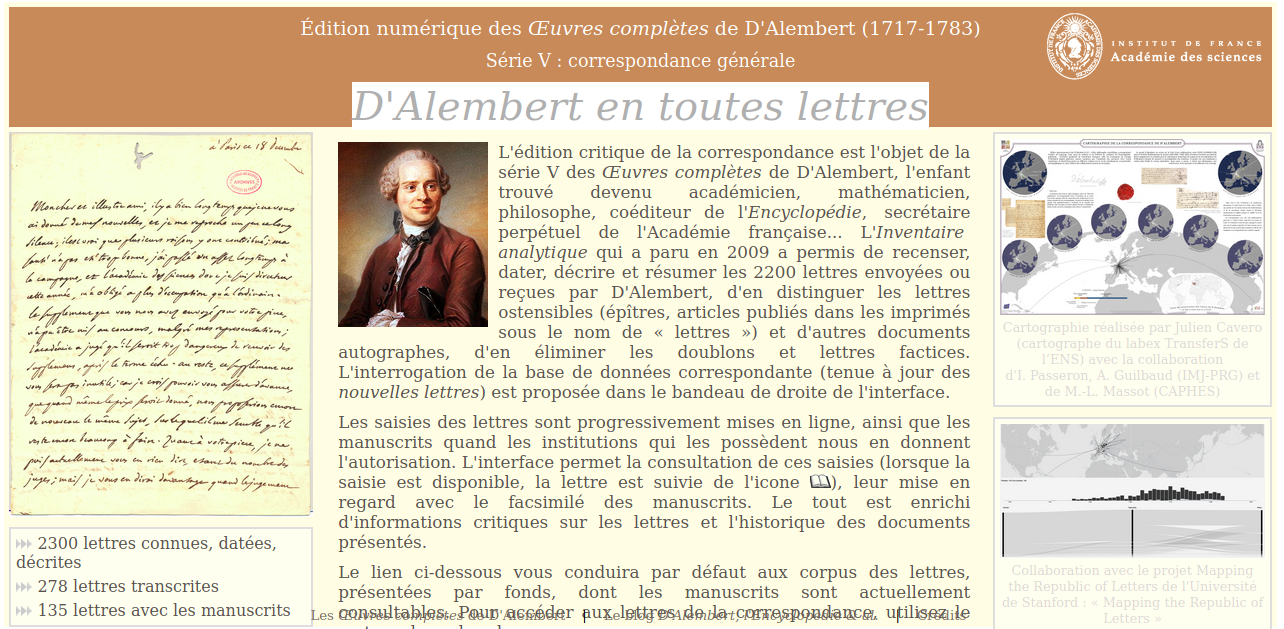
\includegraphics[width=16cm]{images/D_Alembert.png}
    \label{D_Alembert}
\end{figure}

\begin{figure}[ht]
    \centering
    \caption{ Édition numérique de la correspondance de Jean Paulhan, Labex OBVIL}
    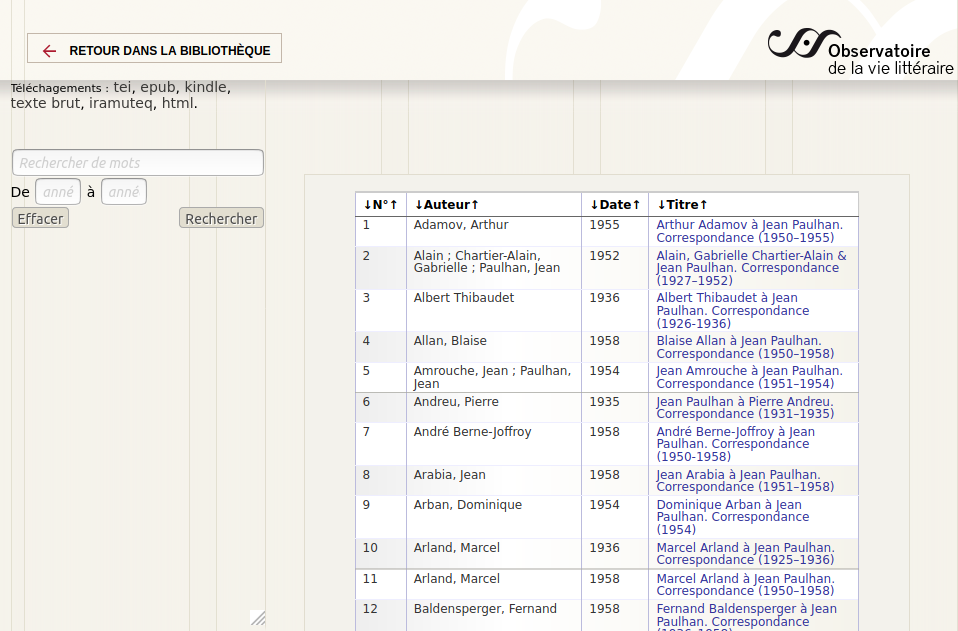
\includegraphics[width=16cm]{images/paulhan_obvil.png}
    \label{paulhan_obvil}
\end{figure}

\begin{figure}[H]
    \centering
    \caption{ Édition numérique de la correspondance de Marc Michel Rey, HUMA-NUM}
    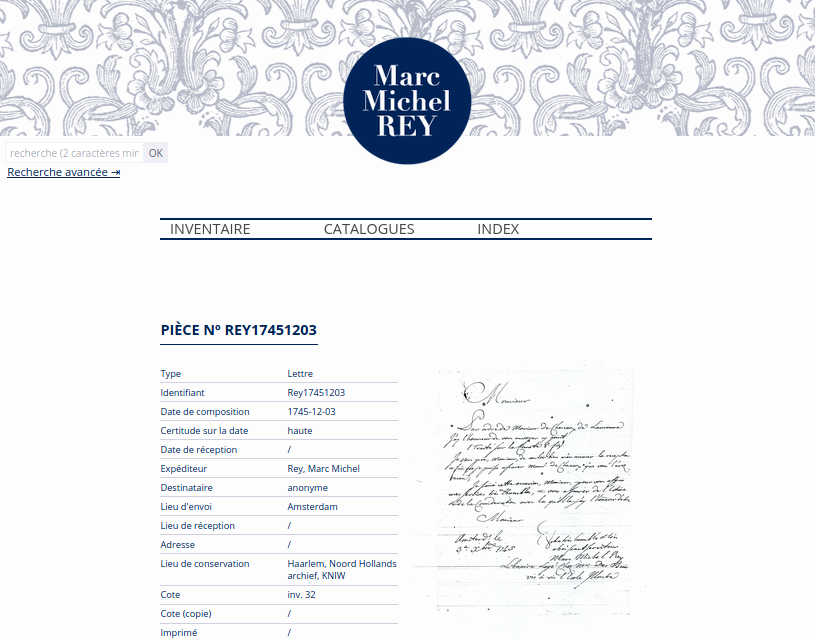
\includegraphics[width=16cm]{images/rey.png}
    \label{rey}
\end{figure}

\begin{figure}[H]
    \centering
    \caption{Accueil de l'édition numérique de la correspondance de Gustave Flaubert, Centre Flaubert}
    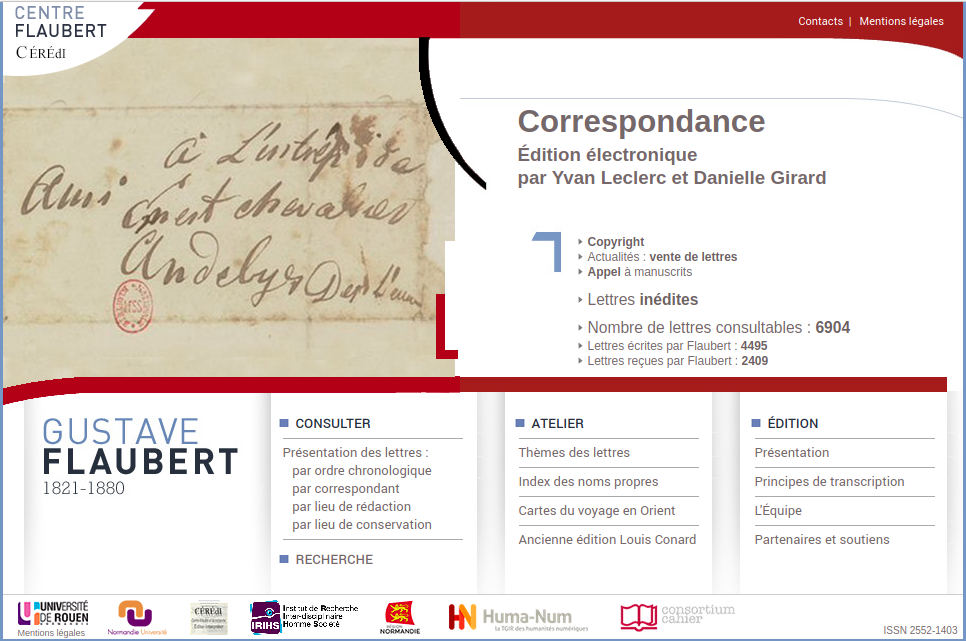
\includegraphics[width=16cm]{images/accueil_flaubert.png}
    \label{accueil_flaubert}
\end{figure}

\begin{figure}[ht]
    \centering
    \caption{Lettre à Théophile Gauthier, Édition numérique de la correspondance de Gustave Flaubert, Centre Flaubert}
    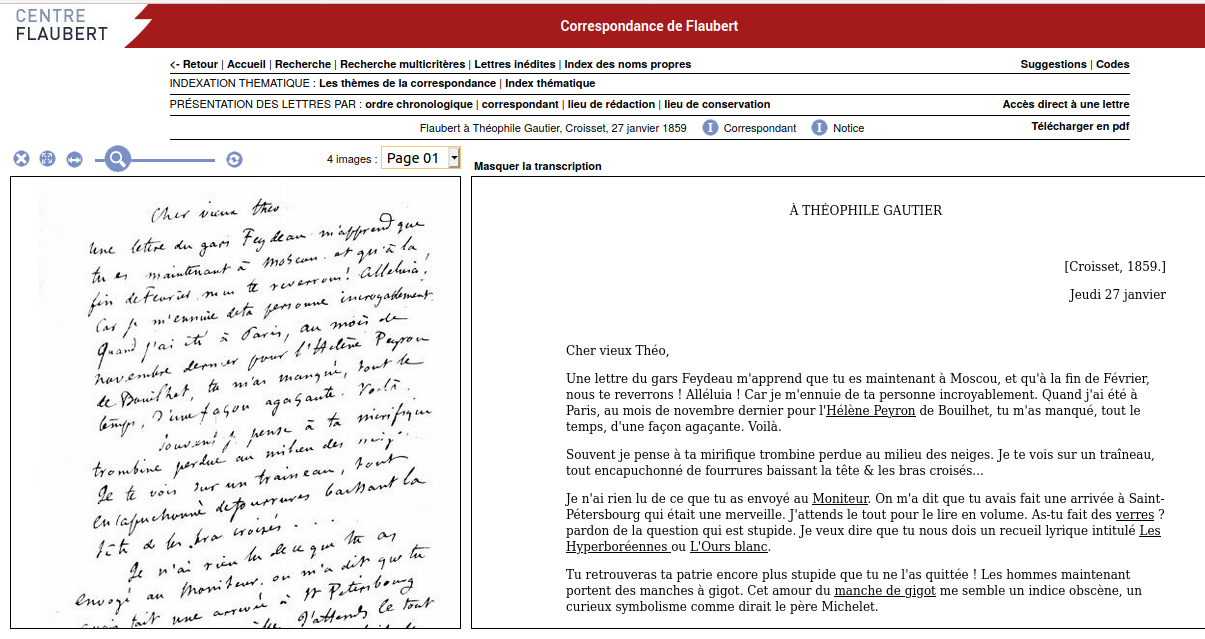
\includegraphics[width=16cm]{images/flaubert_lettre.png}
    \label{flaubert_lettre}
\end{figure}

\begin{figure}[H]
    \centering
    \caption{Lettre Lionel Hauser, Édition numérique de la correspondance de Marcel Proust, Corr-Proust}
    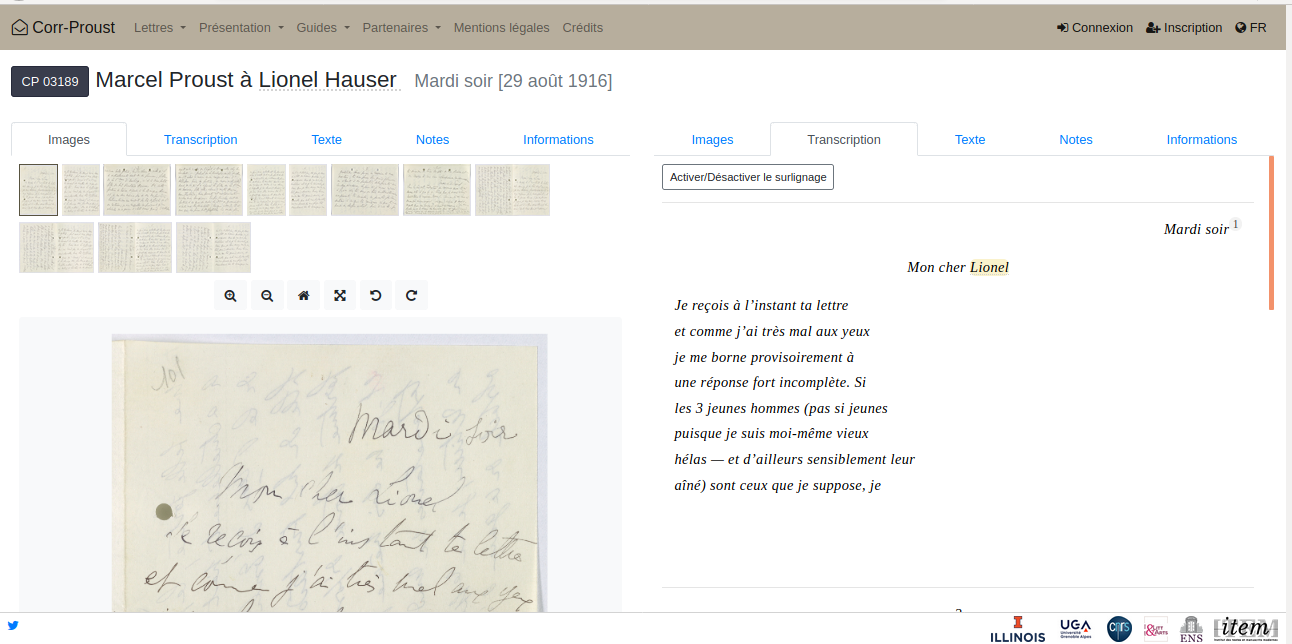
\includegraphics[width=16cm]{images/corr-proust_lettre.png}
    \label{corr-proust_lettre}
\end{figure}

\bigskip
\section{Attentes liées à chaque type de publication}

\begin{figure}[H]
    \centering
    \caption{Grille d’évaluation des publications numériques de corpus d’auteurs}
    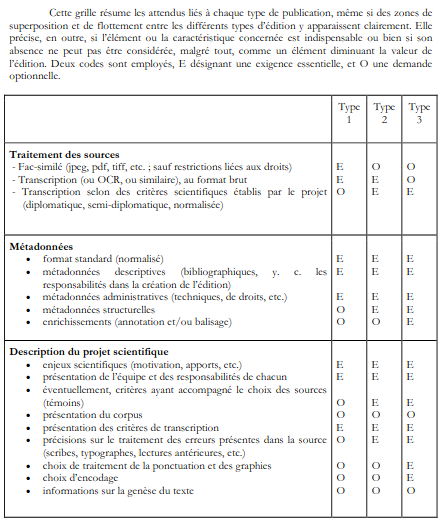
\includegraphics[width=16cm]{images/evaluation_publ_numiq1.png}
    \label{evaluation_publ_numiq1}
\end{figure}

\begin{figure}[H]
    \centering
    \caption{Grille d’évaluation, suite}
    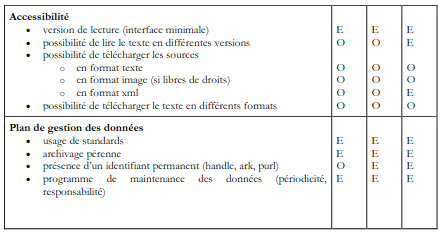
\includegraphics[width=16cm]{images/evaluation_publ_numiq2.png}
    \label{evaluation_publ_numiq2}
\end{figure}

\section{Ébauche d'une arborescence}

\begin{figure}[H]
    \centering
    \caption{Ébauche de l'accueil du futur site d'édition numérique de la correspondance de Frédéric Le Play, CRHXIX}
    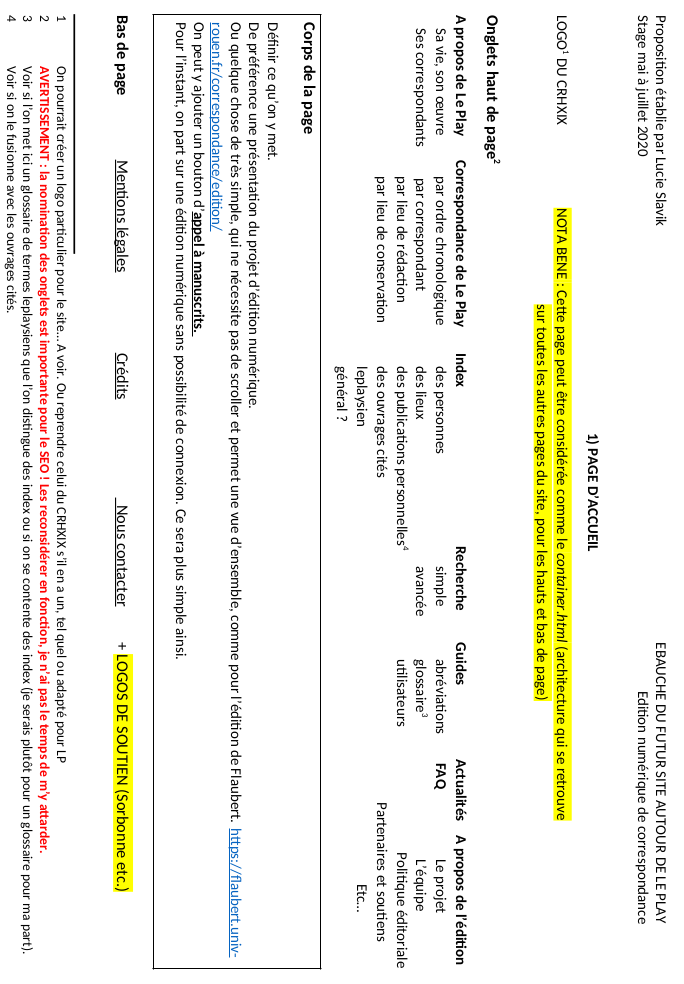
\includegraphics[width=16cm]{images/accueil_site_LP.png}
    \label{accueil_site_LP}
\end{figure}

\chapter{Transcription et Transkribus}

\begin{figure}[ht]
    \centering
    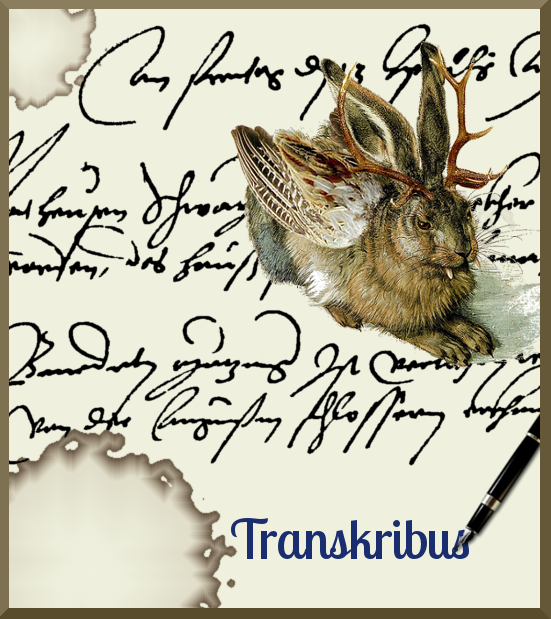
\includegraphics[width=14cm]{images/TRANSKRIBUS.png}
\end{figure}

\section{Les fac-similés}

On peut voir ici quelques exemples des manuscrits que nous avons au CRHXIX. On peut constater les variations d'écriture de Le Play, les différentes qualités de numérisation et les nombreux fonds différents, recélant de la correspondance de Frédéric Le Play.
Nous avons choisi de ne présenter que des lettres écrites par Le Play (excepté celle de Jules Baroche qui illustre nos propos du mémoire). Il faut cependant savoir qu'il existe bien mille lettres de correspondance passive, mais nous n'avons traité que la correspondance active donc c'est celle que nous avons choisi de mettre en valeur.


\begin{figure}[ht]
    \centering
    \caption{Lettre de Jules Baroche à Frédéric Le Play, BIF, Paris)}
    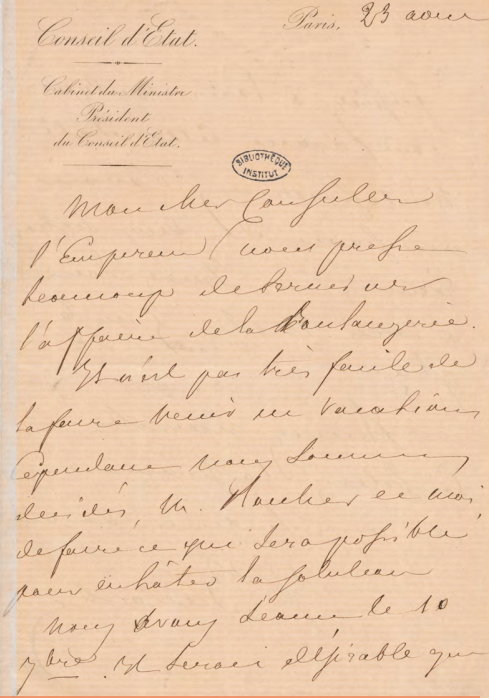
\includegraphics[width=12cm]{images/SIM-MS6062-1Baroche.png}
    \label{SIM-MS6062-1Baroche}
\end{figure}
\begin{figure}[H]
    \centering
    \caption{Lettre de Le Play à Louis de Kergorlay, 1864, Bibliothèque de l'Arsenal, Paris. Exemple typique d'un fac-similé médiocre.}
    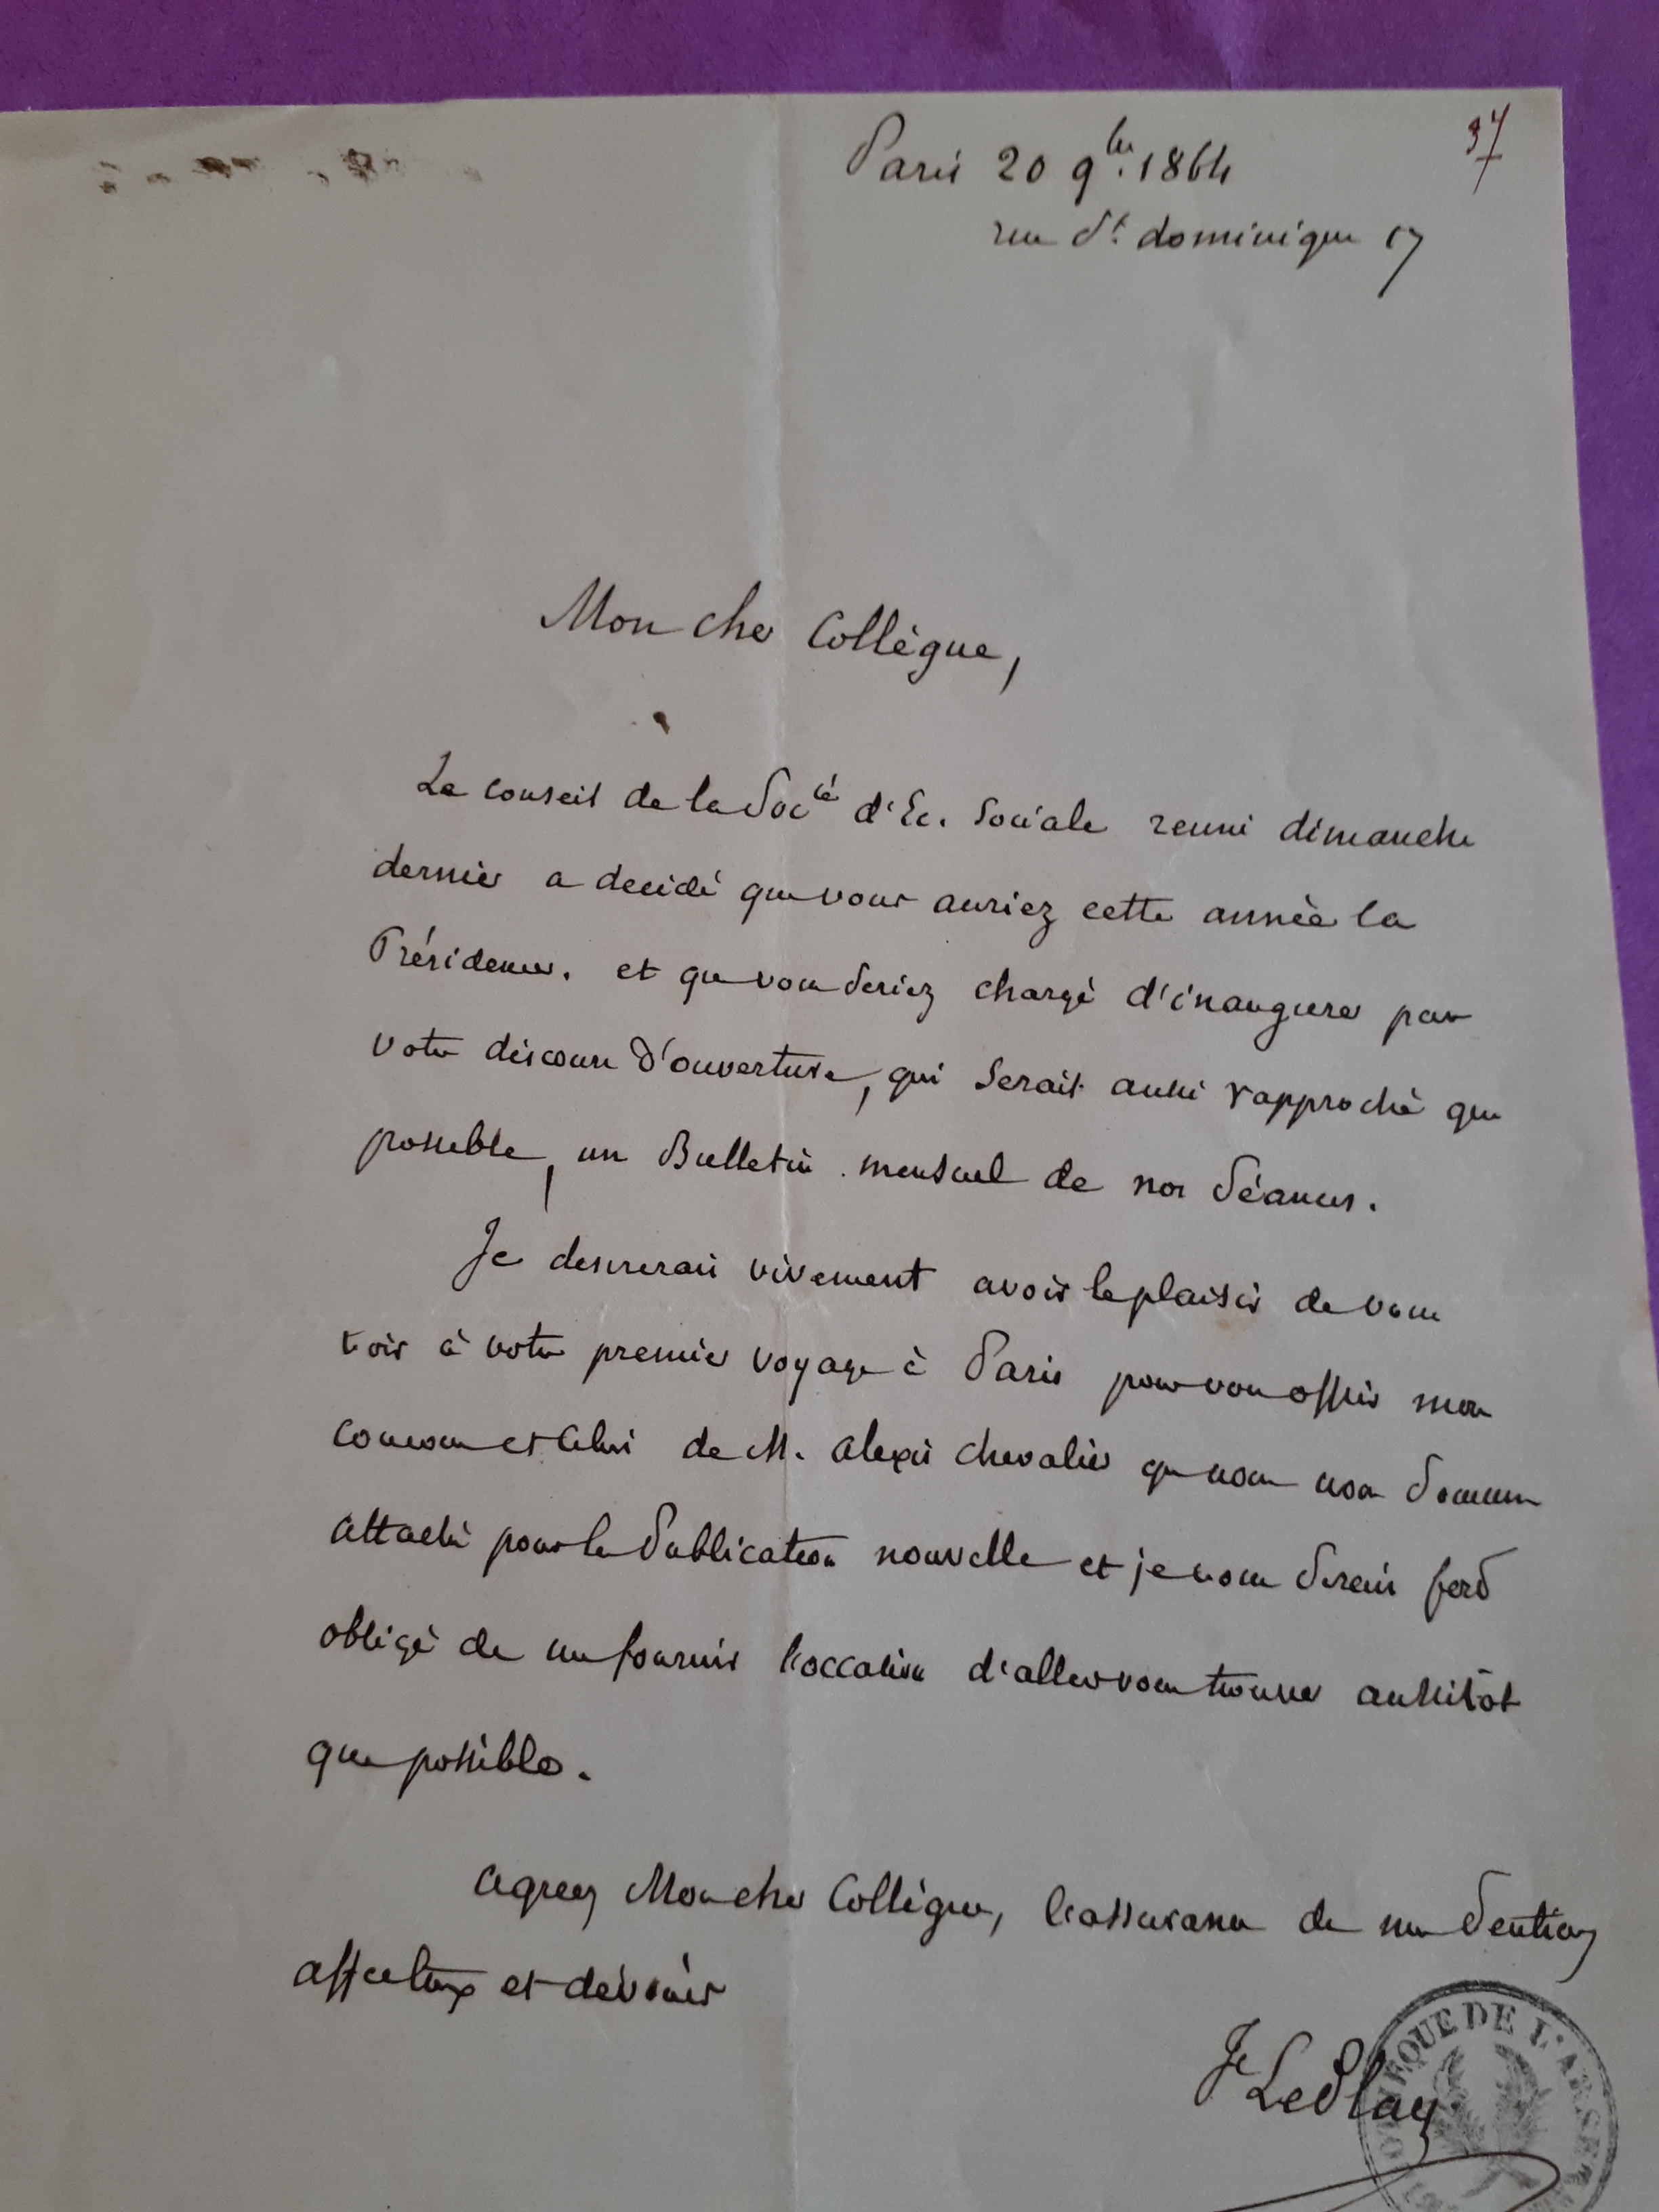
\includegraphics[width=15cm]{images/5MS14112_p37_1p_20sept1864.jpg}
    \label{Kergorlay}
\end{figure}
\begin{figure}[H]
    \centering
    \caption{Lettre de Le Play à Ubaldino Peruzzi, 1857, BNC, FLorence. L'écriture de Le Play est plus penchée, liée et arrondie.}
    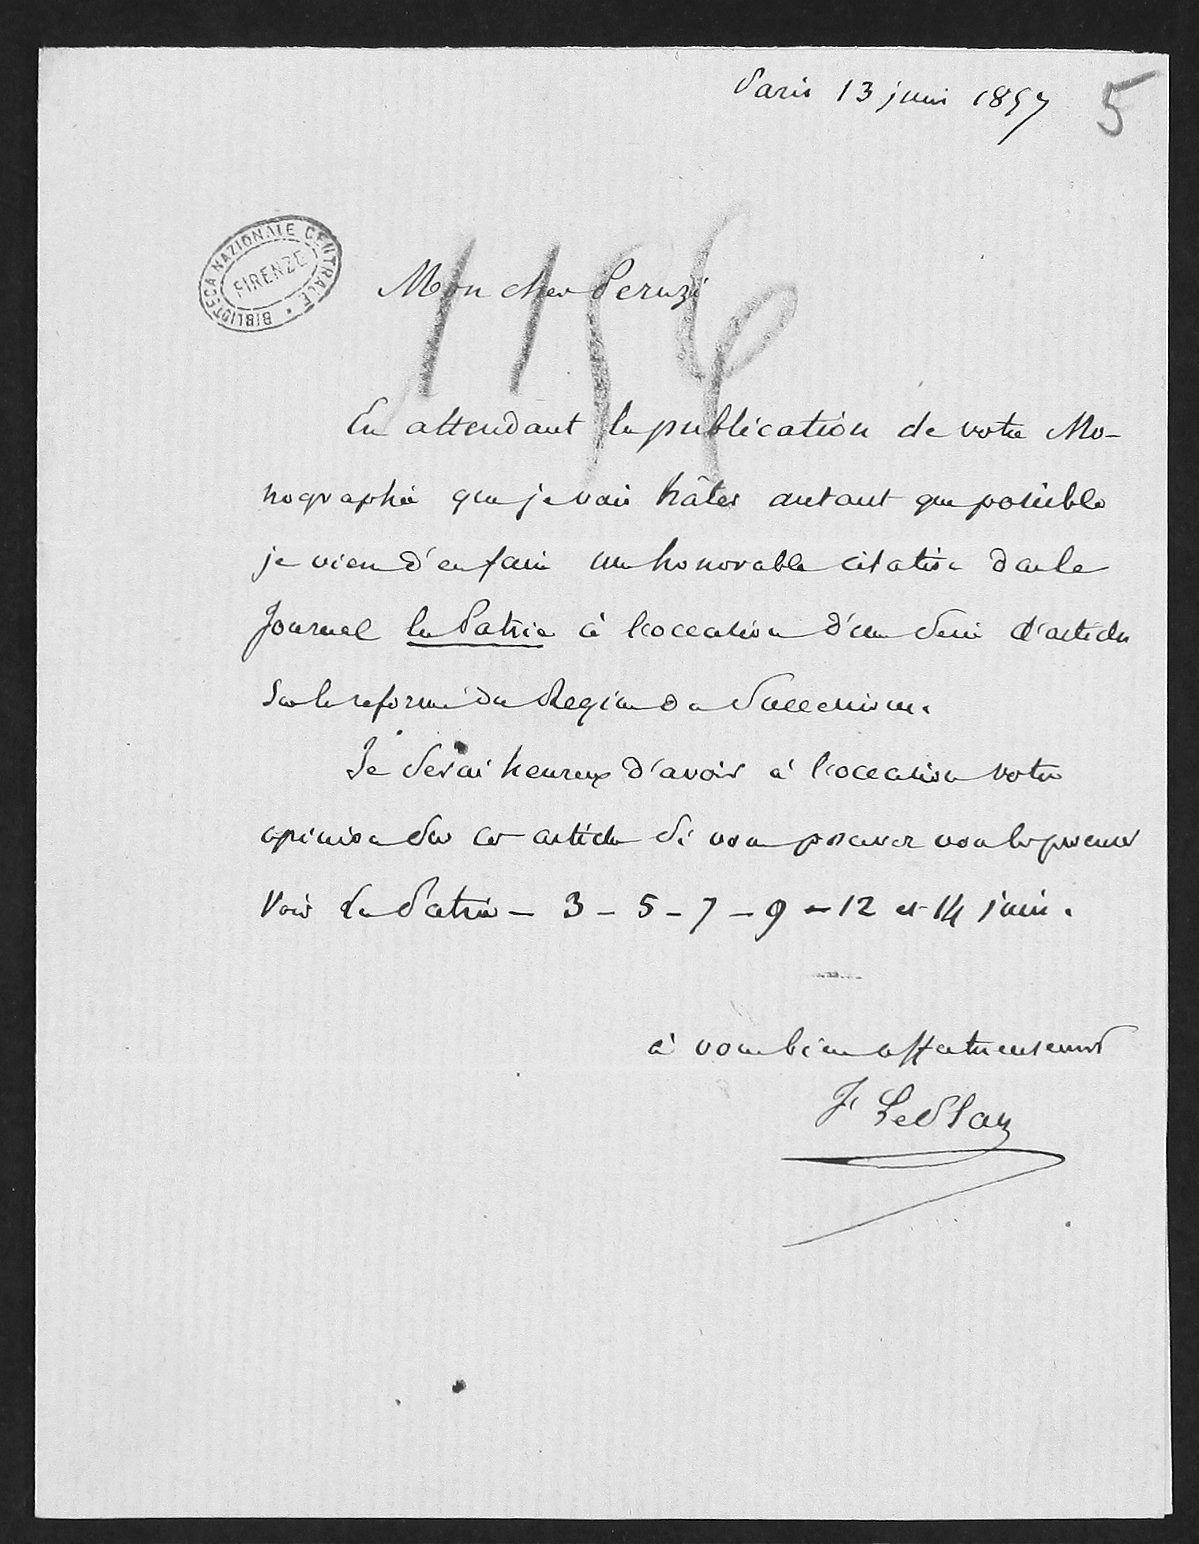
\includegraphics[width=15cm]{images/u peruzzi xxxi ins 37 (7).jpg}
    \label{peruzzi}
\end{figure}
\begin{figure}[H]
    \centering
    \caption{Lettre de Le Play à M\up{gr} Félix Dupanloup, 1873, BNF, Paris. L'écriture de Le Play est très appliquée, plus vieille également, le papier légèrement strié, la plume plus épaisse.}
    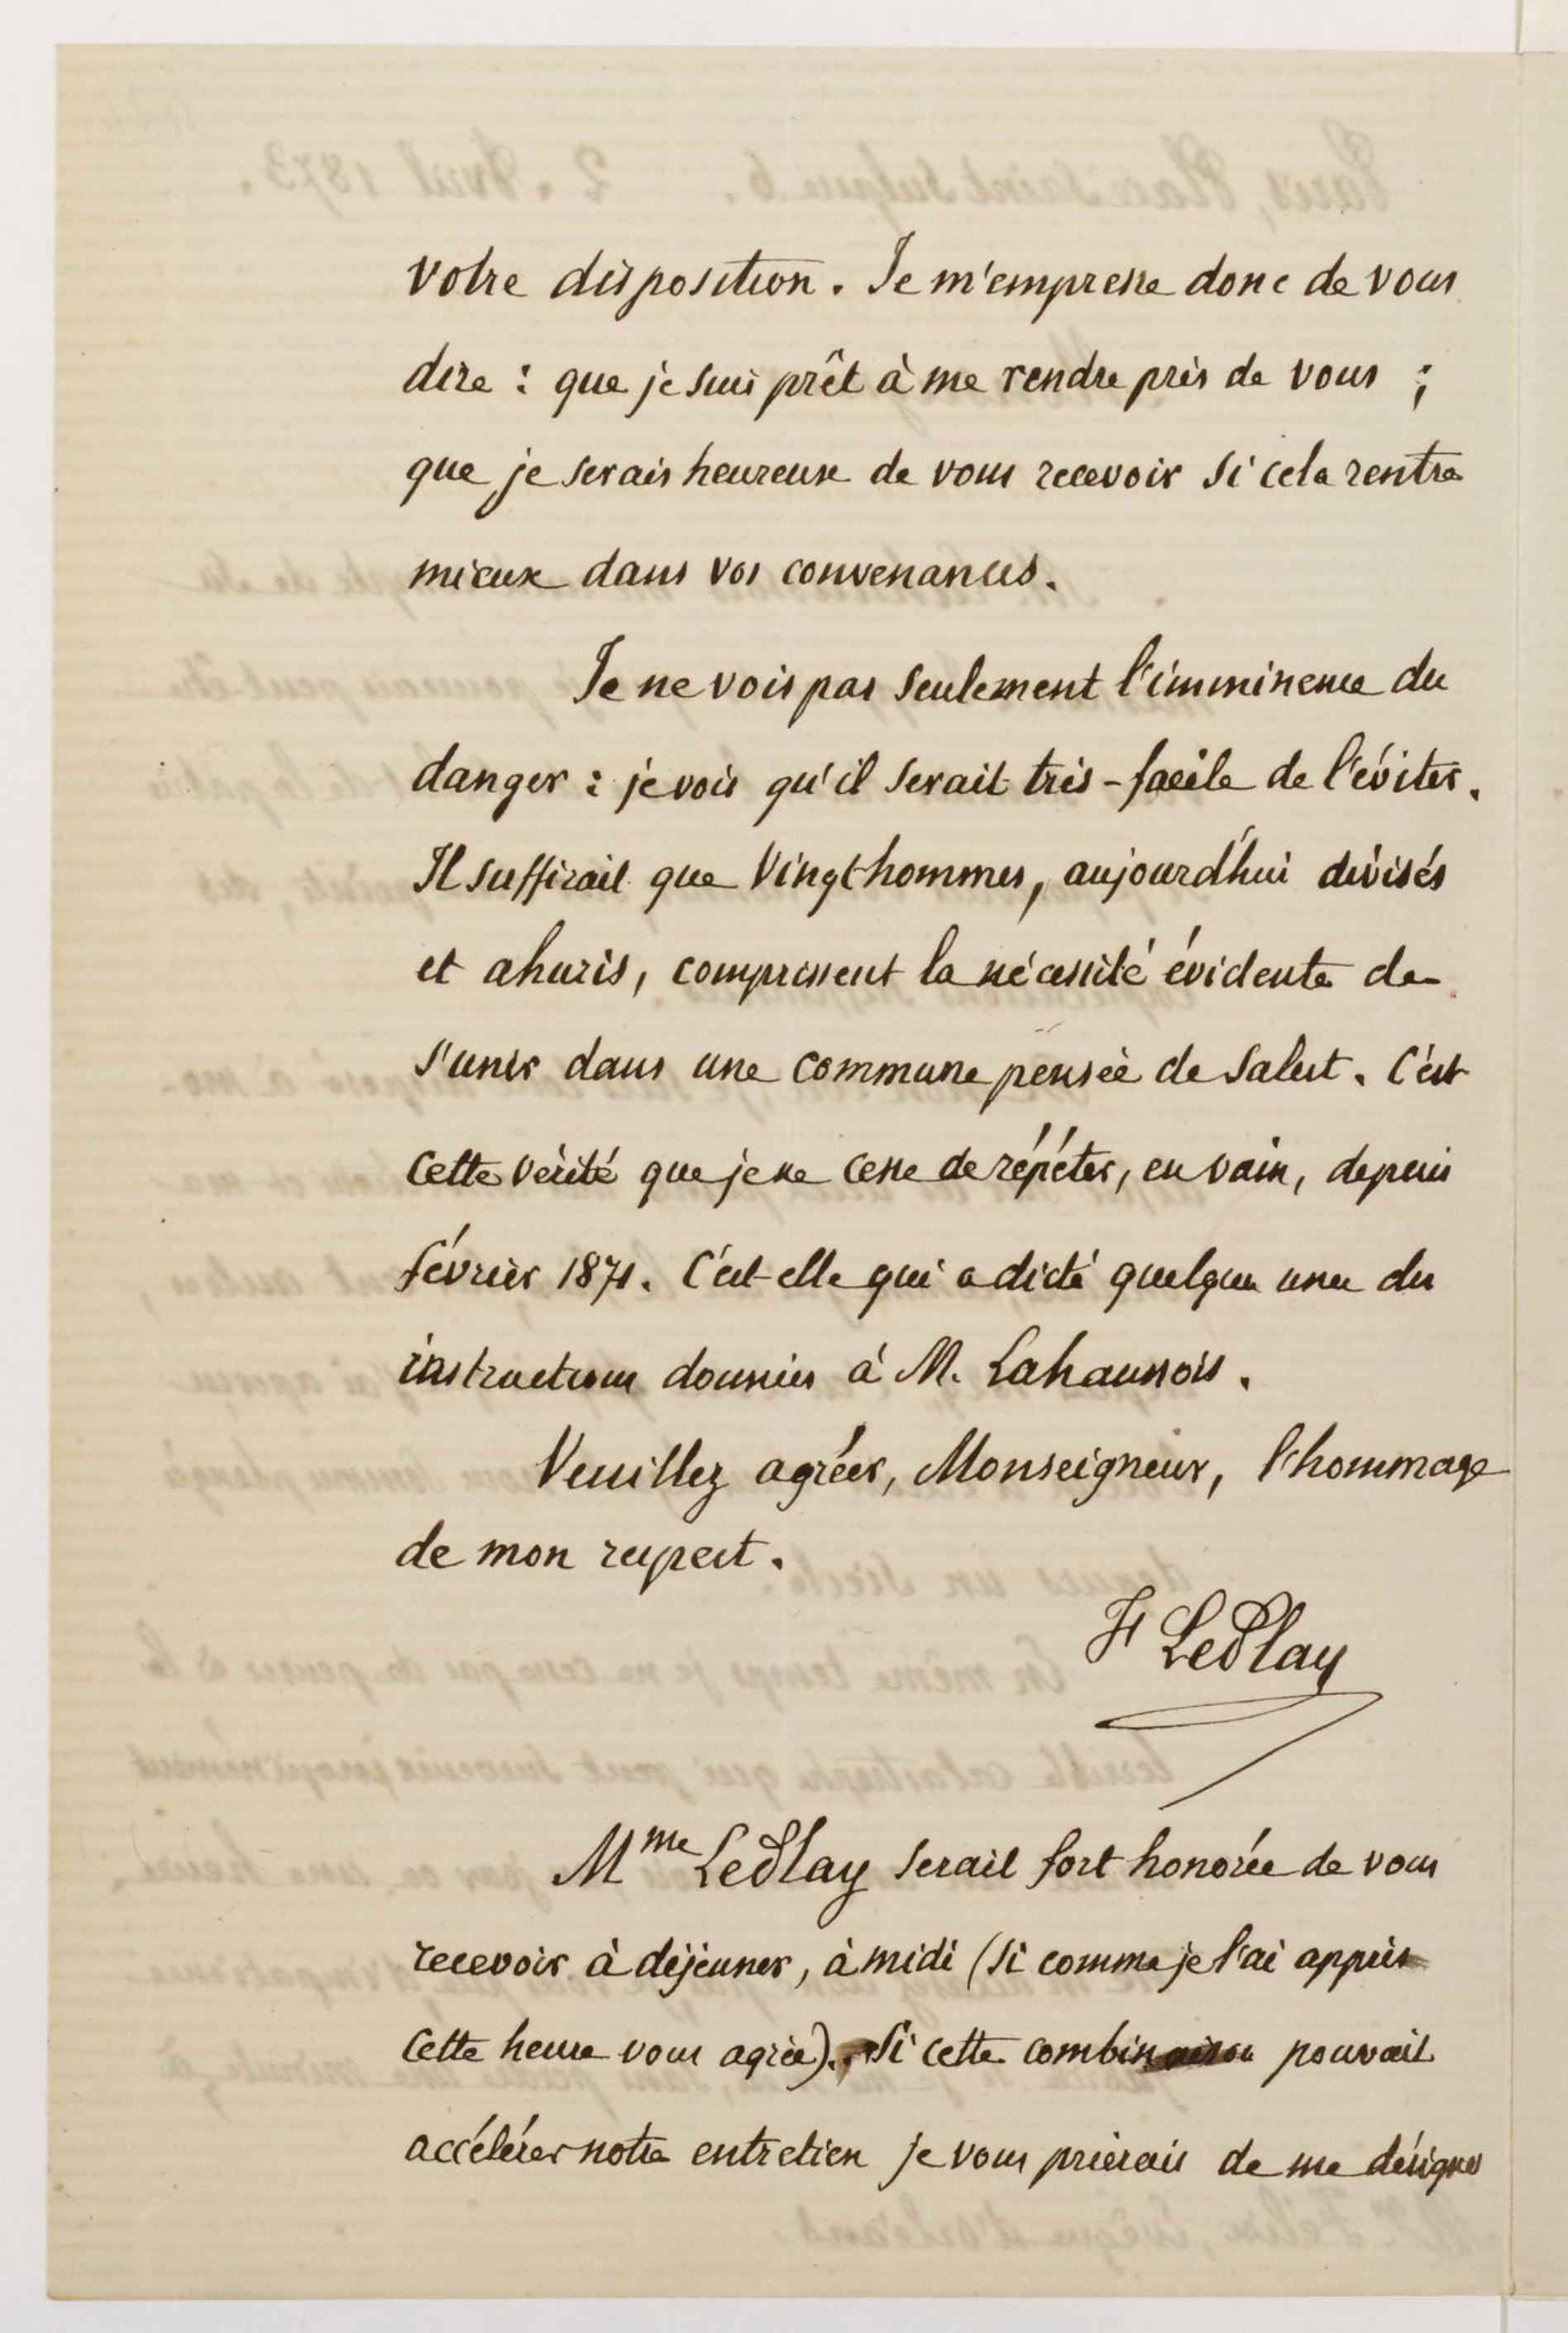
\includegraphics[width=15cm]{images/LPdupanloup2BNF9.jpg}
    \label{dupanloup}
\end{figure}
\begin{figure}[H]
    \centering
    \caption{Lettre de Le Play à Frédéric de Mercey, 1856, BNF, Paris. L'écriture de Le Play est plus hâtive, la plume plus fine.}
    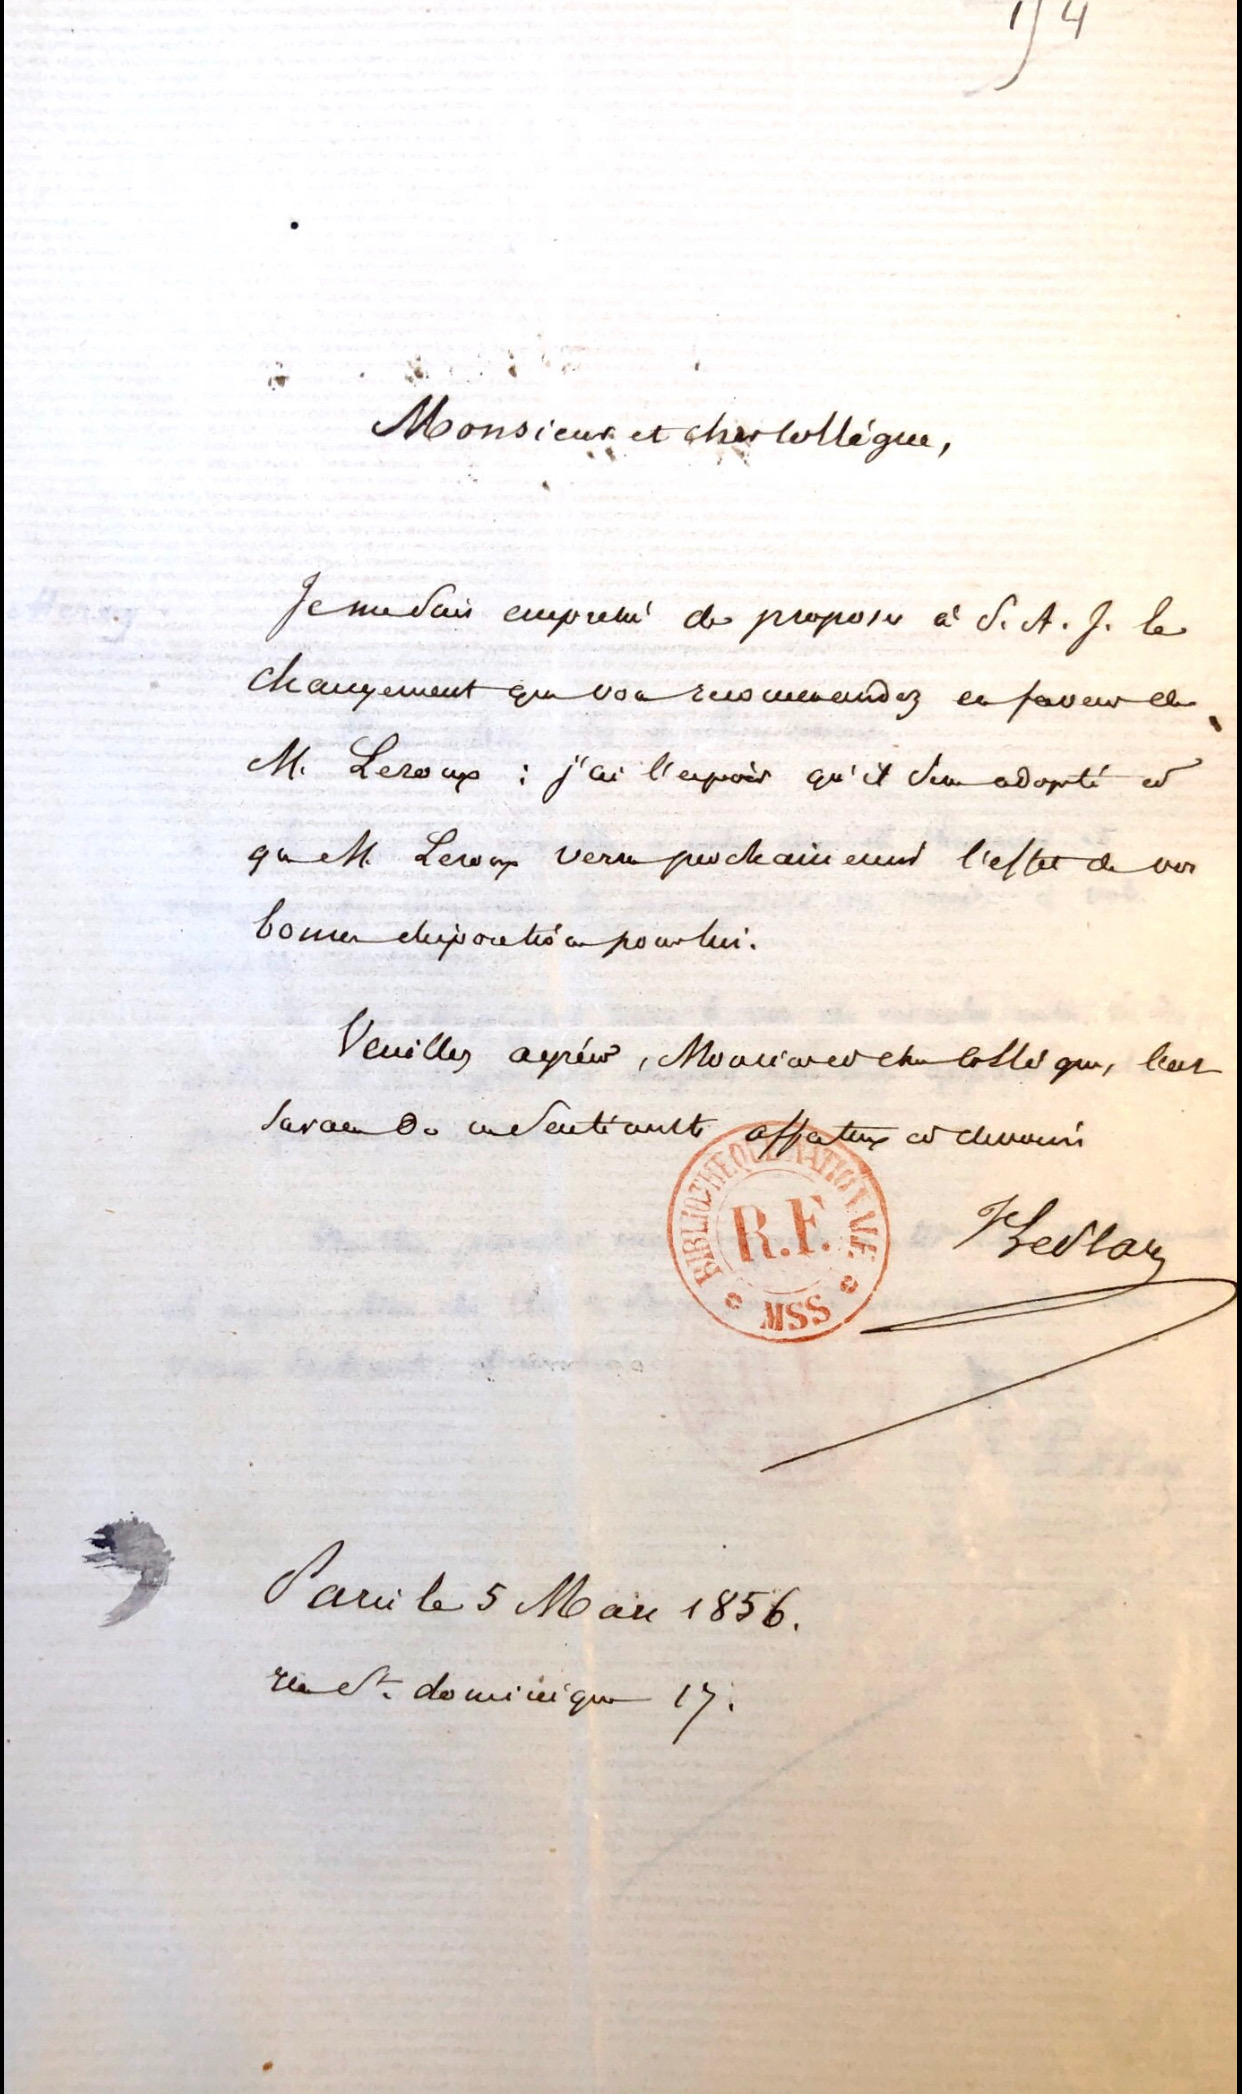
\includegraphics[width=14cm]{images/mercey.JPG}
    \label{mercey}
\end{figure}
\begin{figure}[H]
    \centering
    \caption{Lettre de Le Play son fils Albert, 1865, Château de Ligoure. Le \inquote{A} de Albert s'apparente à un \inquote{a} minuscule.}
    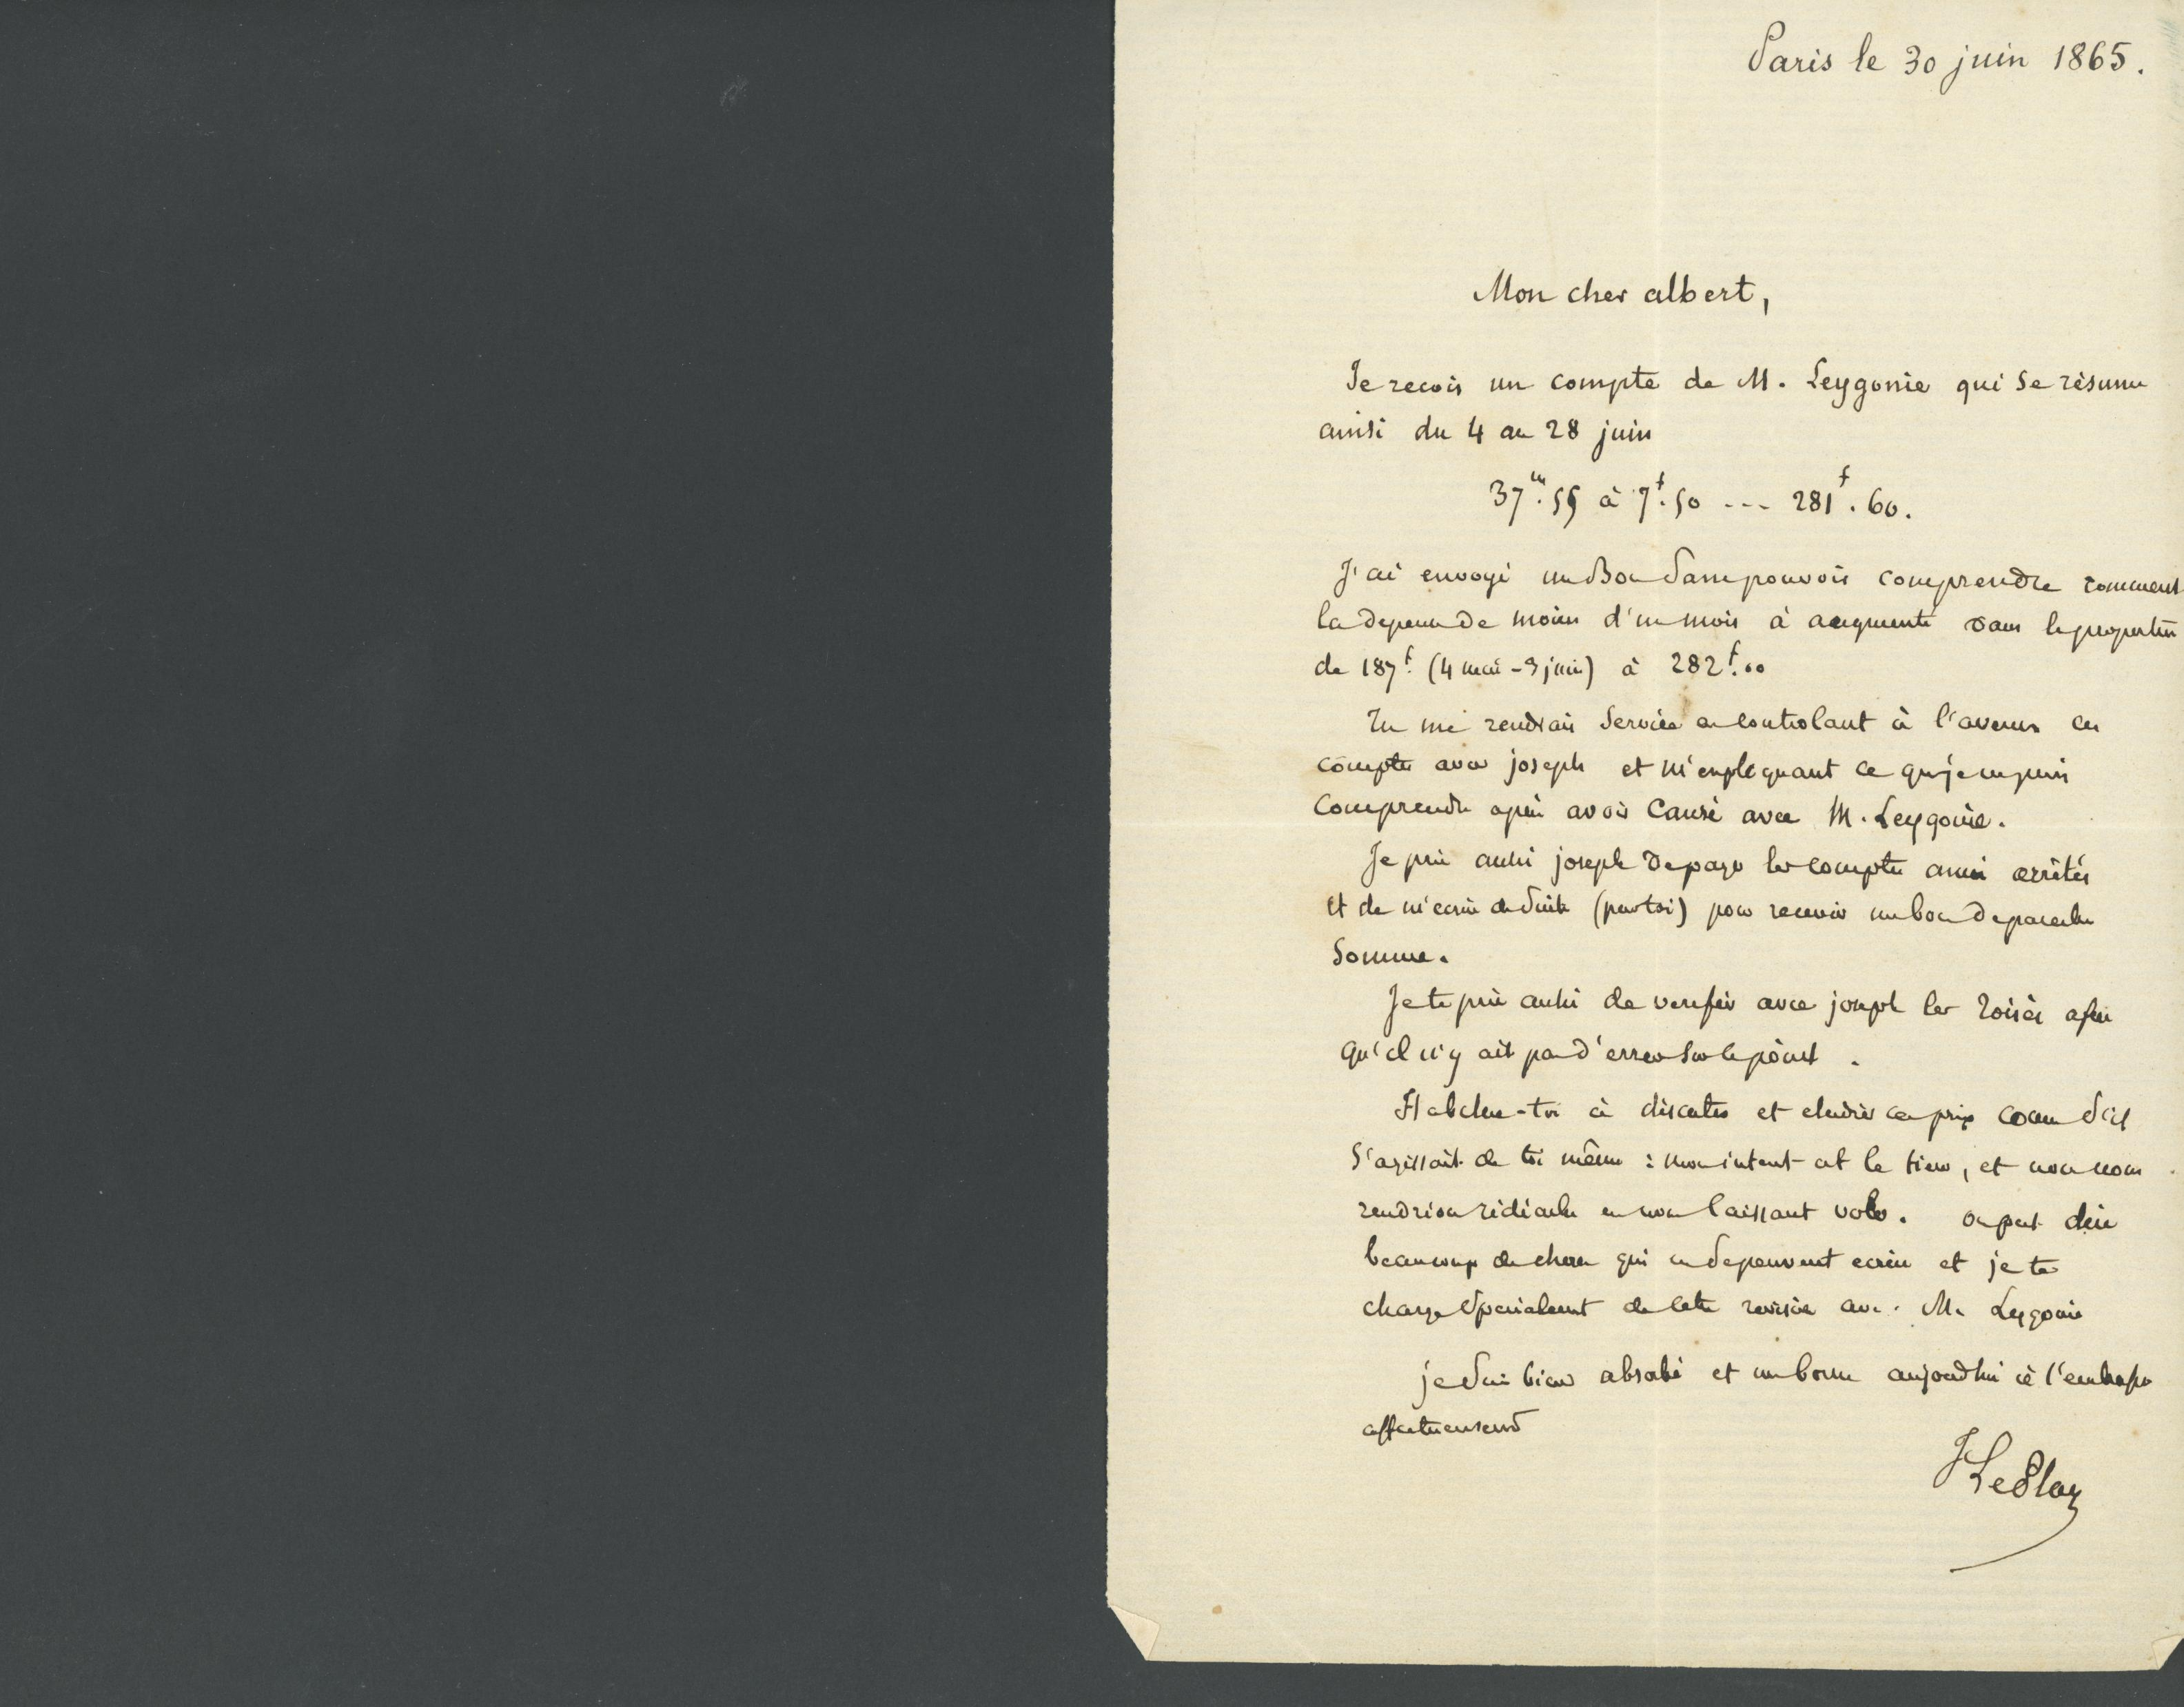
\includegraphics[width=16cm]{images/Frédéric à Albert 001.jpg}
    \label{albertLP}
\end{figure}
\begin{figure}[H]
    \centering
    \caption{Lettre de Le Play Charles de Ribbe, 1869, Musée Arbaud, Aix-en-Provence. L'écriture est plus penchée, moins jeune.}
    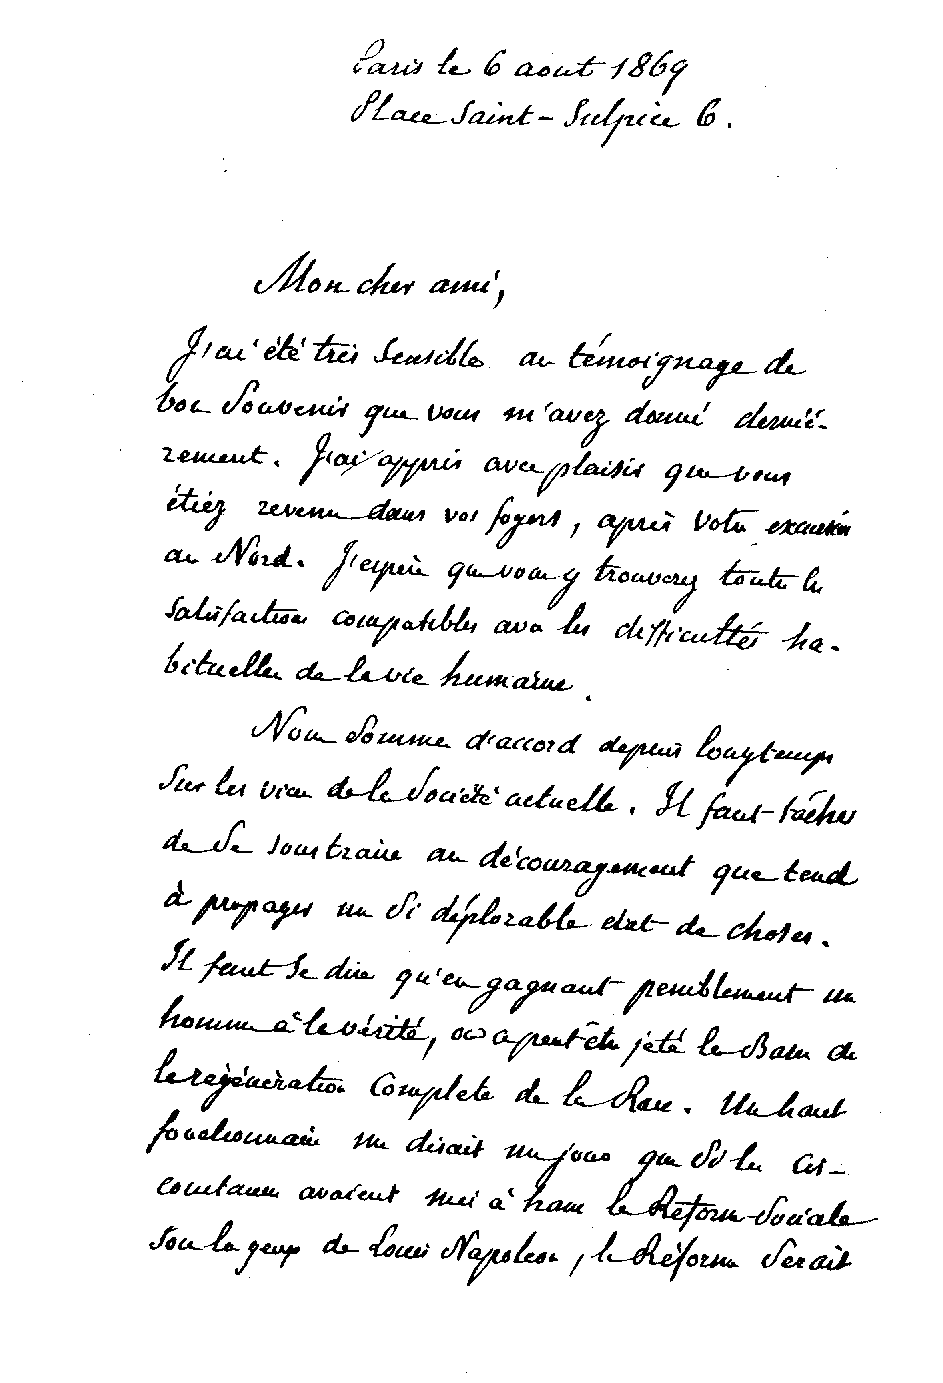
\includegraphics[width=16cm]{images/ribbe.png}
    \label{ribbe}
\end{figure}

\hugeskip 

\section{Chargement des données d'entraînement}

\begin{figure}[H]
    \centering
    \caption{Problème de TR, capture d'écran de Transkribus}
    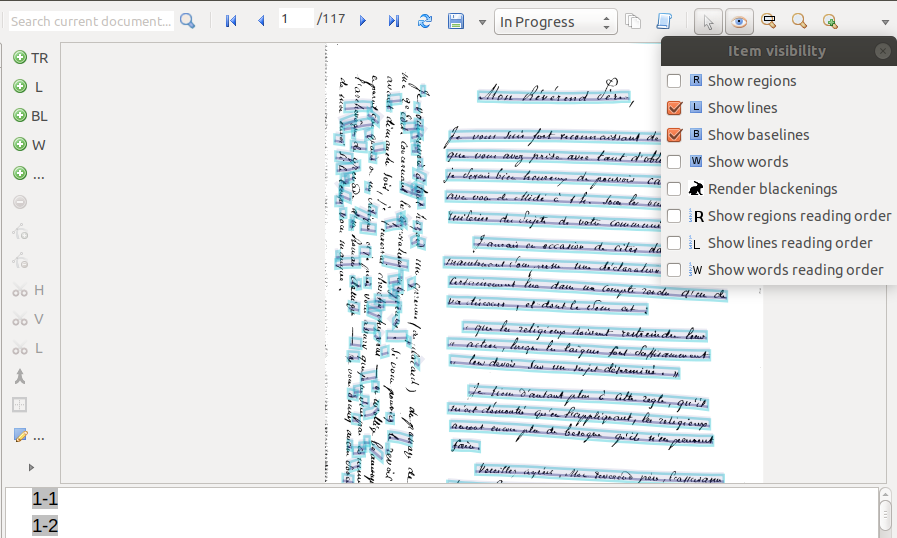
\includegraphics[width=14cm]{images/trTranskribus.png}
    \label{trTranskribus}
\end{figure}

\begin{figure}[H]
    \centering
    \caption{Résolution du problème de TR, deux sens d'écriture, capture d'écran de Transkribus}
    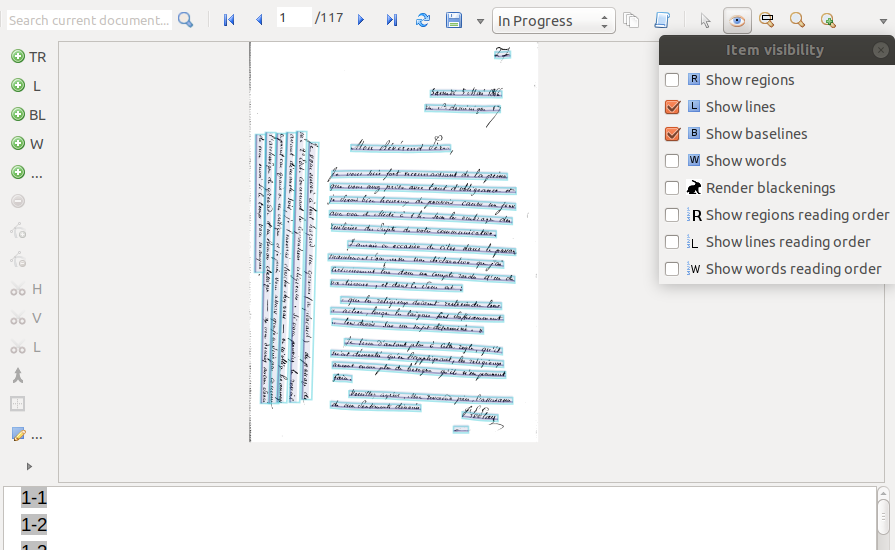
\includegraphics[width=14cm]{images/trCorTranskribus.png}
    \label{trCorTranskribus}
\end{figure}

\section{Schématisation du modèle d’information de Transkribus}

Schéma modèle Transkribus proposé par l'INHA\footnote{\emph{Schéma modèle Transkribus}, Site web de l'INHA, URL : \url{https://skylab.inha.fr/EditionsEnrichies/Documents/Schema-Modele-Transkribus.pdf} (visité le 18/06/2020)}.

\begin{figure}[ht]
    \centering
    \caption{Le modèle de métadonnées Transkribus, INHA}
    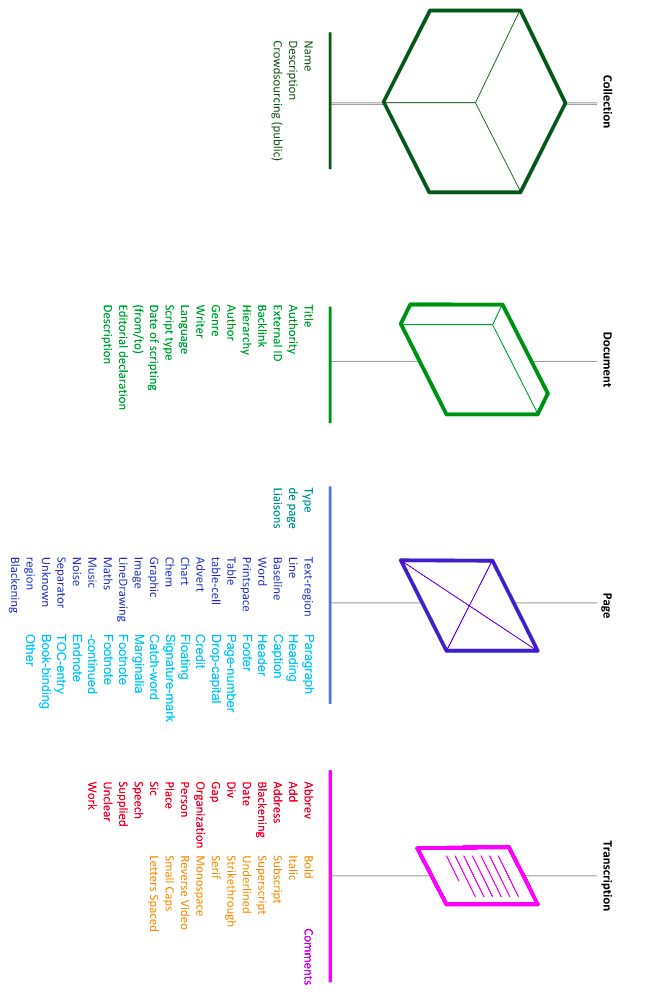
\includegraphics[width=11cm]{images/schema_modele_transkribus_inha1.png}
    \label{schema_modele_transkribus_inha1}
\end{figure}

\begin{figure}[ht]
    \centering
    \caption{La transcription diplomatique numérique via Transkribus, INHA}
    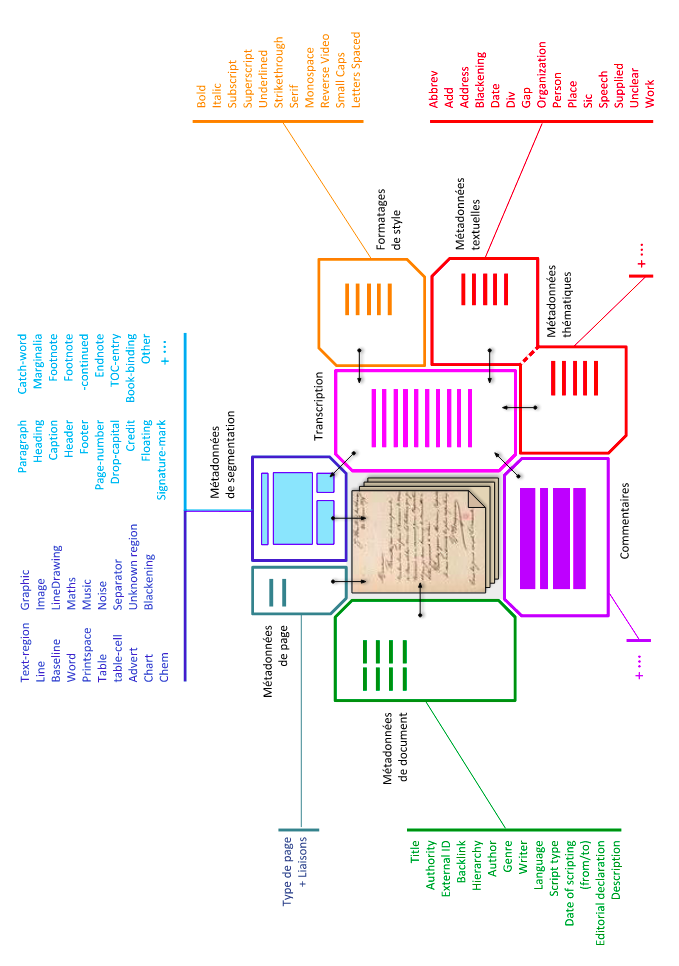
\includegraphics[width=16cm]{images/schema_modele_transkribus_inha2.png}
    \label{schema_modele_transkribus_inha2}
\end{figure}

\begin{figure}[ht]
    \centering
    \caption{\inquote{Cheatsheet} métadonnées Transkribus, INHA}
    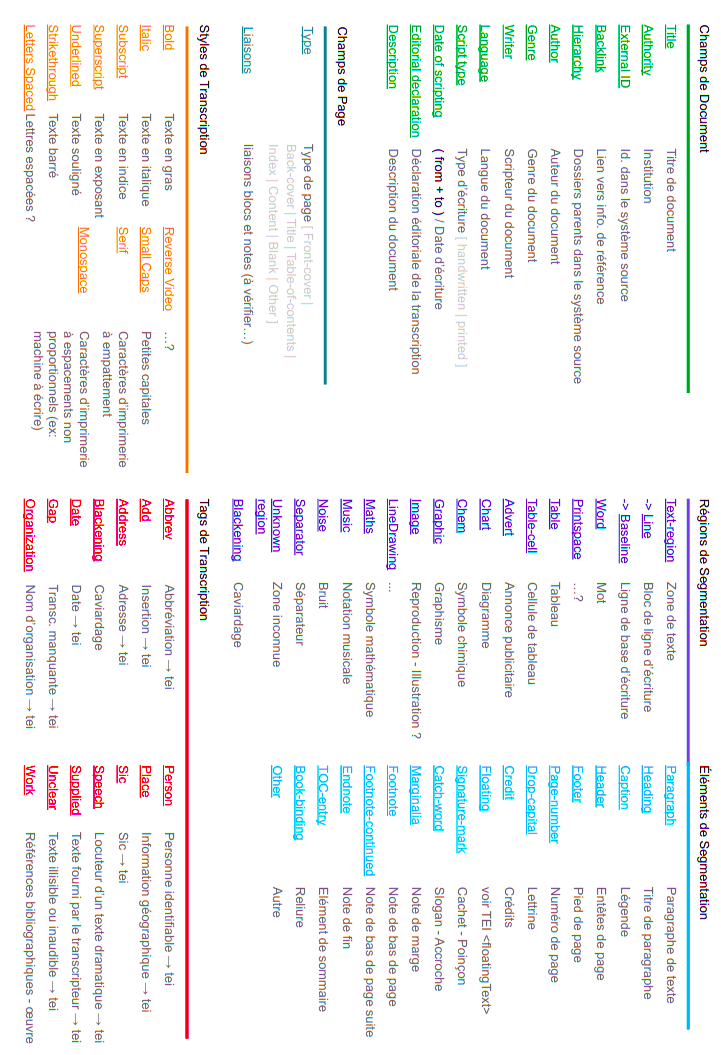
\includegraphics[width=16cm]{images/schema_modele_transkribus_inha3.png}
    \label{schema_modele_transkribus_inha3}
\end{figure}

\chapter{L'encodage en XML-TEI}
\section{Les index}

\begin{figure}[H]
    \centering
    \caption{L'index de vocabulaire leplaysien, capture d'écran de l'ODD}
    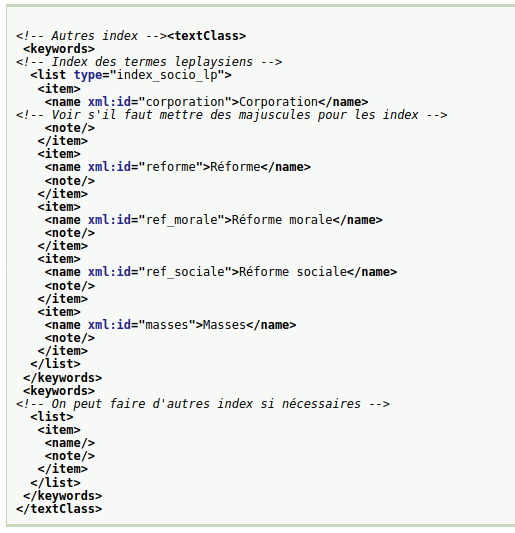
\includegraphics[width=14cm]{images/indexLP.png}
    \label{indexLP}
\end{figure}

\chapter{Livrables du CRHXIX}

Pour mieux se repérer dans les livrables, il est conseillé de consulter le fichier \citecode{arborescence\_detaillee.txt} qui donne une arborescence détaillée des livrables, ou alors, pour embrasser tout dans une rapide vue d'ensemble, on consultera de préférence le fichier intitulé \citecode{arborescence.txt} qui ne fait pas le détail pièce par pièce. 

\section{\citecode{CRHXIX/rapport\_fin\_stage\_CRHXIX.pdf}}

Ces livrables ont été faits au cours de notre stage au CRHXIX qui recouvrait une période de 31,5 jours de travail.
Dans l'ensemble, les 15 premiers jours ont été consacrés à la prise en main du projet et le travail sur Transkribus, les 15 autres ont été employés à l'établissement du cahier des charges et de récits utilisateurs, dans une forme d'ébauche, permettant ainsi d'arriver au schéma XML-TEI et à l'ODD.


Pour avoir une petite vue d'ensemble du travail réalisé au cours de ce stage, il sera bon de lire le fichier \citecode{rapport\_fin\_stage\_CRHXIX.pdf} qui fait une synthèse des tâches accomplies.

\section{\citecode{CRHXIX/1-inventaires}}

\begin{itemize}
    \item Pour mieux comprendre ce qu'a été le travail de prise en main du projet, nous avons mis le fichier excel \citecode{Inventaire\_cor\_LP.xlsx} fait d'après le premier inventaire de 2005-2006 réalisé par Stéphane Baciocchi et Antoine Savoye dans \emph{La correspondance de Le Play, une source pour l'histoire des sciences sociales}, Stéphane Baciocchi in \emph{Les Études Sociales / Cairn.info}, 142-143-144 (II-2005-2006).
    \item Nous y joignons cet inventaire \citecode{Inventaire\_LP\_plain\_text\_gallica.odt} dans lequel nous avons fait mention des archives numériques en notre possession lors de ce stage.
\end{itemize}

A noter : ces documents sont encore à un stade de travail et devraient être perfectionnés. Ils ont surtout servi à la prise en main du projet à court terme.

\begin{figure}[ht]
    \centering
    \caption{Aperçu de l'inventaire de prise en mains du projet, capture d'écran, mai 2020.}
    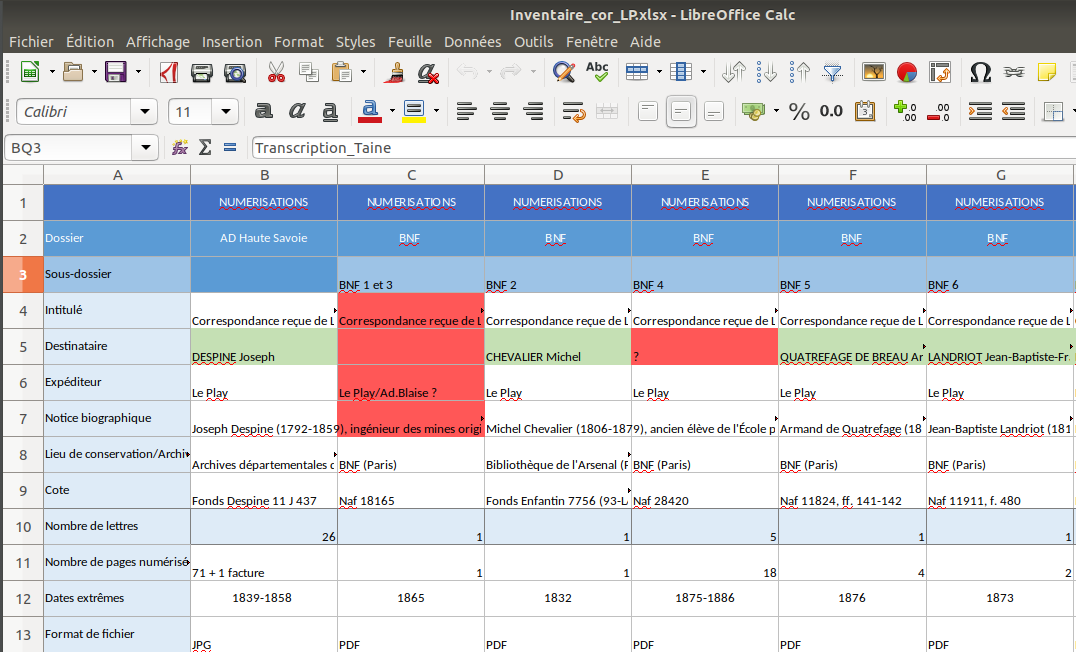
\includegraphics[width=14cm]{images/inventaire.png}
    \label{inventaire}
\end{figure}
La couleur rouge mentionne les points obscurs et les données incertaines.

\section{\citecode{CRHXIX/2-transcriptions}}

On trouve dans ce dossier un échantillon d'une transcription réalisée par la stagiaire M. F. On peut y lire en note de bas de page les autres suggestions faites à la lecture de certains mots qui ne nous semblaient pas cohérents selon le contexte. 
Nous avons fait cela très occasionnellement, le but de notre stage étant surtout de gérer la partie technique. On voit ici l'avantage de notre formation initiale en sciences humaines qui nous permet de comprendre le fond et d'avoir une réflexion à son sujet (et donc de pouvoir corriger certaines erreurs) alors que nous sommes en train de travailler sur la partie plus technique. Cela peut être également un frein car l'important reste aussi la gestion de la partie technique.
On peut voir un exemple de ces ponctuelles corrections à la page 11 de cette transcription \citecode{LePlay\_Loyson\_MF.pdf}.

\section{\citecode{CRHXIX/3-trankribus}}

Ce dossier comprend les tutoriels que nous avons réalisés pour la prise en main de Transkribus.
Cela permettra à l'équipe du CRHXIX de continuer notre travail après notre départ, afin d'éviter le \inquote{facteur d'autobus} (en anglais \inquote{\emph{bus factor}}) provoqué par l'absence de partage d'informations et de compétences.

\begin{itemize}
    \item Les membres de l'équipe du CRHXIX pourront donc, grâce au fichier\\ \citecode{Tuto1\_préparation\_des\_donnees\_transkribus.pdf} apprendre à préparer les données en vue de l'entraînement d'un modèle expliqué dans le fichier\\ \citecode{Tuto2\_entraînement\_du\_modèle.pdf}.
    \item Le fichier \citecode{Tuto3\_application\_du\_modele.pdf} explique ensuite comment l'appliquer pour transcrire automatiquement.
Ils pourront donc, s'ils estiment que c'est pertinent, outre le fait de continuer à entraîner le modèle Le Play, en créer d'autres sur les correspondants les plus importants.
Et quoi qu'il en soit, ils pourront prendre en main Transkribus pour les simples transcriptions ce qui sera déjà un bon point pour le projet.
\item Enfin, le fichier \citecode{Tuto4\_exportation\_transkribus.pdf} explique comment exporter les données du serveur Transkribus à notre ordinateur. En effet, il est important de garder la main sur nos données.
\end{itemize}


En guise de complément à ce tutoriel, se trouve dans le dossier \citecode{export\_test} un test d'export des données de Transkribus vers l'ordinateur. Il est à noter que les fichiers ne sont pas encore nommés dans la forme qu'ils prendront, telle qu'on a pu la constater dans le dossier numérisation. 
\begin{itemize}
    \item On trouve ainsi dans le dossier \citecode{BNF9enJPG}, comprenant les lettres de Le Play à Monseigneur Félix Dupanloup, un export des fichiers transcrits en XML-TEI avec les numérisations correspondantes. 
    \item De même pour les lettres de Le Play à Charles de Ribbe \citecode{LP\_à\_Charles\_de\_Ribbe1} : on trouve toujours un fichier XML-TEI regroupant l'ensemble des lettres, ici\\ \citecode{LP\_à\_Charles\_de\_Ribbe\_tei.xml}, puis dans le dossier \citecode{page} un fichier XML-TEI par page transcrite (et non par lettre transcrite). Il est intéressant de constater ici le test qui a été fait : nous avons utilisé, notamment à la page 4, les \emph{tags} Transkribus et nous avons ensuite exporté en XML pour voir ce que cela donnerait. Or, ces tags se traduisent par des balises et attributs qui ne sont visibles que dans le fichier XML général et non par page. Par ailleurs, leur nommage est souvent invalide. Tout ceci est développé dans le mémoire.
    \item Le dossier \citecode{LP\_à\_Charles\_de\_Ribbe2} comprend l'export d'une sélection plus restreinte de lettres mais avec des \emph{tags} plus poussés. Il a été fait plus récemment. Il comprend également un export en \citecode{.txt}, ce qui permet une comparaison avec l'export .\citecode{xml}.
    \item Dans le dossier \citecode{Set\_entrainement\_le\_play}, l'export a été fait dans plusieurs formats. Pour les fichiers \citecode{.docx}, \citecode{.pdf}, \citecode{.xlsx}, cela n'a pas fonctionné. En revanche, les formats \citecode{.txt} et \citecode{.xml} ne présentent pas d'anomalie. Or, c'est ce qui nous intéresse donc l'expérience s'avère concluante.
\end{itemize}


Le dossier Transkribus comprend également un rapport réalisé sur l'apport de Transkribus au projet.
Ce rapport \citecode{Point\_Transkribus.pdf}, rédigé à la moitié de notre stage, a été transmis au CRHXIX en juin. Il a été partiellement repris dans notre mémoire avec des réflexions mises à jour selon le recul que nous avons actuellement.


\section{\citecode{CRHXIX/4-cahier\_des\_charges}}

Une partie importante de la mise en pratique du projet a été l'établissement d'un cahier des charges. C'est un bien grand mot étant donné que nous n'avons pas eu le temps de le mener à terme. 
C'est donc plutôt un rapport menant à la réalisation d'un futur cahier des charges qui sera vraiment réalisé par la suite.

En complément de cette ébauche de cahier des charges, on trouve un fichier excel nommé \citecode{users\_stories\_LP\_V3.ods} dans lequel sont écrits des récits utilisateurs ou \emph{users stories} permettant de mieux cerner les attentes des futurs visiteurs et utilisateurs de l'édition numérique et donc d'adapter notre édition à leurs besoins. 
Là encore, ces US gagneraient à être améliorés.

Nota : à chaque fois, on trouve le nommage V2 ou V3 à la fin des noms de fichiers. Cela signifie que nous avons fait plusieurs versions et que nous mettons la dernière (V1~= version 1, V2~= version 2, V3~= version 3 et ainsi de suite).

\section{\citecode{CRHXIX/5-site}}

Il a fallu penser le site de l'édition numérique.
C'est encore une ébauche de réflexion qui sera continuée par un membre de l'équipe du CRHXIX.

On trouve ici :
\begin{itemize}
    \item Dans le dossier \citecode{pages} les pages du site telles qu'elles ont été pensées pour l'édition numérique de la correspondance de Le Play.
    \item Le fichier \citecode{architecture\_site\_LP.JPG} présente l'architecture. Les numéros qui y sont inscrits renvoient aux fichiers du dossier \citecode{page}
\end{itemize}


\section{\citecode{CRHXIX/6-index}}

Une fois que l'on s'est fait une idée plus précise des attentes des utilisateurs et des besoins du site, il s'agit d'entreprendre la mise en oeuvre technique pour répondre à ces attentes.
Un des points importants est la réalisation d'index.
Il a été convenu pour les choix éditoriaux que nous ferions plusieurs index~: un index pour les noms de personnes, un pour les noms de lieux, un pour les grands événements, un pour les noms d'organisation, un pour les ouvrages cités, un pour les termes leplaysiens ou tout au moins sociologiques.
Pour ce dernier, il a été nécessaire de mener une réflexion plus importante pour savoir en amont quels termes nous indexerions. Pour cela, nous avons sélectionné certains mots qui nous paraissaient importants dans les lettres que nous avions déjà croisées, et nous avons soumis cet index au Professeur Antoine Savoye.
Le fichier nommé \citecode{Vocabulaire leplaysien - mots à ajouter.doc} contient les mots que nous lui avons soumis et qui ont été retenus. 
Il ne nous a pas paru intéressant de mettre les autres index dans les livrables.
En revanche, nous les avons mis dans leur forme provisoire, tels qu'ils seront utiles pour l'encodage TEI dans le dossier suivant.


\section{\citecode{CRHXIX/7-index\_tei}}

Ce dossier comprend les index en cours de constitution, tels qu'ils apparaîtront dans les lettres encodées en XML-TEI.
À chaque index correspond un fichier recensant les noms dans leur forme finale en XML-TEI. Cela permettra à la personne qui prendra la suite, d'une part d'avoir un modèle à suivre, d'autre part de pouvoir lister chaque nom rencontré et de se contenter de faire un copier/coller lors de l'encodage suivant.

On trouve donc ici :
\begin{itemize}
    \item l'index des noms d'événement~: \citecode{index\_evenements\_tei.pdf}
    \item l'index des termes leplaysiens et sociologiques~: \citecode{index\_leplaysien\_tei.pdf}
    \item l'index des noms de lieu~: \citecode{index\_lieux\_tei.pdf}
    \item l'index des noms d'organisation~: \citecode{index\_organisations\_tei.pdf} 
    \item l'index des noms d'ouvrages : \citecode{index\_ouvrages\_tei.pdf}
    \item l'index des noms de personnes et personnages : \citecode{index\_personnes\_tei.pdf} 
\end{itemize}

En outre, une recension des formes normalisées de correspondants à renseigner dans le \citecode{<teiHeader>} se trouve dans le fichier intitulé \citecode{index\_correspondants\_teiHeader.pdf}.

On aurait pu faire un index pour aider les transcripteurs à remplir les informations sur les origines du document, mais nous avons estimé que le fichier\citecode{ xxxx\_base.xml} (voir le point 8 sur la tei ) fait pour chacun des documents suffisait.

\section{\citecode{CRHXIX/8-tei}}

Dans ce dossier se trouvent les premiers essais d'encodage qui ont permis de réaliser ensuite l'ODD. 
\begin{itemize}
    \item le dossier \citecode{lp\_dupanloup\_xml} comprend les premiers essais d'encodage en XML-TEI.
  Ils sont nommés respectivement \citecode{lp\_dupanloup\_bnf-l1.xml} et \citecode{lp\_dupanloup\_bnf-l2.xml} (\citecode{lp} pour leplay, on indique toujours l'auteur des lettres en premier ; \citecode{dupanloup} pour le destinataire, \citecode{bnf} pour le lieu de conservation du fonds, \citecode{lxxx} pour le numéro de la lettre. Ici, les lettres 1 et 2).
  Le fichier \citecode{lp\_dupanloup\_bnf\_base.xml} comprend tous les éléments communs aux manuscrits écrits de Le Play à Dupanloup. Il sert de base à l'encodage de chacune des lettres.
    \item même principe pour le dossier \citecode{lp\_ribbe\_arbaud\_xml}
    \item le fichier \citecode{essai\_tei\_correspondance\_CRHXIXv2.xml} est un essai (très perfectible) d'encodage qui a aidé à la réflexion d'encodage en vue de l'ODD.
    \item  le fichier \citecode{Tuto\_XML-TEI\_CHRXIX.pdf} est un tutoriel qui a été réalisé pour le CRHXIX par nos soins, afin d'aider l'équipe du Centre dans les futurs encodages.
\end{itemize}



\section{\citecode{CRHXIX/9-odd}}

Les réflexions sur l'encodage en XML-TEI aboutissent à l'ODD (\emph{One Document Does it all}).
Ce dossier comprend :
\begin{itemize}
    \item l'ODD en html \citecode{ODD\_LEPLAY\_V1.html}
    \item un dossier \citecode{LP\_testODD} qui contient les test réalisés sur un fichier XML lié à l'ODD par un schéma relaxNG. 
\end{itemize}

L'ODD est perfectible. En quinze jours travaillés, nous n'avons pas eu le temps d'avoir une vue assez complète des milliers de lettres en notre possession, mais c'est déjà un bon point de départ pour l'encodage, et nous pensons qu'il ne devra pas être beaucoup modifié. Mais il devra l'être un peu, c'est inévitable.

\chapter{Livrables du Labex OBVIL}


Le stage au Labex Obvil recouvre une totalité de 20 jours travaillés.

Le fichier \citecode{rapport\_fin\_stage\_OBVIL.pdf} est le rapport qui a été écrit en fin de stage dans le but d'informer le chef de projet, Monsieur Glenn Roe, du travail accompli.

On trouvera sur Github les rapports qui ont été faits au quotidien à partir d'une certaine date, et une bonne partie des fichiers réalisés : \url{https://github.com/OBVIL/elicom/tree/master/extraction\_cor\_stage2020}. 
Néanmoins, il nous a paru plus clair d'en faire une sélection ici et de l'expliquer de la même manière que nous l'avons fait pour le CRHXIX, afin de garder une cohérence de moyens.

\section{Les fichiers XML-TEI}

Le dossier intitulé \citecode{extraction\_cor\_stage2020} rassemble l'ensemble des livrables d'Obvil.
\begin{itemize}
    \item \citecode{extraction\_cor\_stage2020/cor\_lamartine} : les fichiers en lien avec la correspondance d'Alphonse de Lamartine. Total de 97 fichiers XML-TEI extraits et corrigés.
    \item \citecode{extraction\_cor\_stage2020/cor\_lamennais} : ceux qui traitent de la correspondance de l'Abbé Félicité de Lamennais. Total de 204 fichiers. Certains sont nommés a, b, c car ils ont dû être divisés a posteriori. Nous avons corrigé 80 fichiers. Il faut encore corriger 124 fichiers, à savoir les fichiers 164 à 195, 2 à 9, 17 à 99.
    \item \citecode{extraction\_cor\_stage2020/cor\_proudhon} : ceux concernant Pierre-Joseph Proudhon. Total de 87 fichiers extraits et corrigés.
\end{itemize}



\section{Organisation des dossiers}

Les dossiers sont toujours organisés de la même manière au sein de chaque dossier \citecode{cor\_nomDuCorrespondant}, reflet de ce travail plus systématique.
Dans chacun on trouve les dossiers suivants :

\subsection{\citecode{corpus}}

Il rassemble d'une part le PDF extrait sur Gallica et dont nous nous servons pour repérer la mise en page et les passages versifiés afin de bien encoder, d'autre part l'extraction de l'OCR de ce même volume, en HTML. L'HTML a été corrigé par nos soins pour en assurer la validité.


\subsection{\citecode{\emph{script}}}

Comme son nom l'indique, il renferme le \emph{script} Python qui permet de passer de l'OCR HTML à un fichier XML par lettre. Le squelette est commun pour les auteurs, mais adapté aux variations de chacun.
Il est de qualité inégale. Le temps nous a manqué pour parfaire le premier \emph{script} réalisé (Lamartine).


\subsection{\citecode{dump}}

Il contient les extractions XML corrigées (sauf pour Lamennais où seulement une partie est corrigée, comme indiqué dans le rapport).

\subsection{\citecode{remarques}}
Sur Github, on peut voir les rapports écrits au jour le jour mais qui n'ont pas grand intérêt. 
Nous avons mis ici les fiches faites au fur et à mesure de notre travail, mais qui ont un aspect souvent de réflexion et d'ébauche, car ils ont été faits selon le cours de nos réflexions, qui sont peut-être plus avancées aujourd'hui. Certains des questionnements ont été résolus.
On trouve également des index de noms normalisés pour permettre de faire par la suite des copier/coller et avancer plus vite dans la correction des fichiers XML-TEI.
